\documentclass{slnotes}

\newcommand{\cdotplus}{\mathbin{\substack{\cdot\\+}}}
\newcommand{\pluscdot}{\mathbin{\substack{+\\\cdot}}}

\begin{document}
%\chapter{Powers of 2}
%\begin{tabular}{llll}
%\toprule
%\(n\) & \(2^n\) & \(n\) & \(2^n\) \tabularnewline
%\midrule
%-10 & 0.0009765625 & 1 & 2 \tabularnewline
%-9  & 0.001953125  & 2 & 4 \tabularnewline
%-8  & 0.00390625   & 3 & 8 \tabularnewline
%-7  & 0.0078125    & 4 & 16 \tabularnewline
%-6  & 0.015625     & 5 & 32 \tabularnewline
%-5  & 0.03125      & 6 & 64 \tabularnewline
%-4  & 0.0625       & 7 & 128 \tabularnewline
%-3  & 0.125        & 8 & 256 \tabularnewline
%-2  & 0.25         & 9 & 512 \tabularnewline
%-1  & 0.5          & 10 & 1024 \tabularnewline
%15 & 32768         & 16 & 65536 \tabularnewline
%20 & 1048576       & 24 & 16777216 \tabularnewline
%30 & 1073741824 \tabularnewline
%31 & 2147483648    & 32 & 4294967296 \tabularnewline
%\bottomrule
%\end{tabular}
\chapter{Number systems}
\(n\) bits can represent \(2^n\) values.

To convert a decimal to binary, divide by 2 repeatedly; the remainders form the answer, with the first being the LSB. To convert a fraction to binary, multiply by 2 repeatedly; the carries form the answer, with the first being the MSB.

\sldef{Sign-and-magnitude}. One bit for sign, remaining bits for magnitude. Range is \([-(2^{n-1}-1), 2^{n-1}-1]\). Two zeroes. To negate, flip sign bit.

\sldef{1's complement}. MSB is sign. Range is same as above. Two zeroes. To negate, flip all bits: \(-x = 2^n - x - 1\). When adding, if there is a carry out of MSB, add 1 to the result.

\sldef{2's complement}. MSB is sign. Range is \([-2^{n-1}, 2^{n-1}-1]\). Only one zero. To negate, flip all bits and add 1: \(-x = 2^n - x\). When adding, ignore carry out of MSB.

Overflow has occurred if the operands have the same sign but the result has a different sign.

\sldef{Excess}. Excess-\(n\) means \(-n\) is represented as 0, etc.

\sldef{IEEE-754}. 32-bit: 1-bit sign, 8-bit exponent (excess-127), 23-bit mantissa. 64-bit: 1-bit sign, 11-bit exponent (excess-1023), 52-bit mantissa. When the exponent field is all 0, the mantissa is denormalised, and the actual exponent is the bias plus 1 (i.e. \(-126\) for 32-bit).
\chapter{MIPS}
\tablehead{\toprule Pseudo & Realised\tabularnewline}
\begin{xtabular}{ll}
\midrule
\code{move \$x, \$y} & \code{add \$x, \$y, \$zero}\tabularnewline
\midrule
\code{li \$x, 0xXXXXYYYY} & \begin{tabular}{@{}l@{}}\code{lui \$at, 0xXXXX} \tabularnewline
\code{ori \$x, \$at, 0xYYYY}\end{tabular}\tabularnewline
\midrule
\code{blt \$x, \$y, z} & \begin{tabular}{@{}l@{}}\code{slt \$t, \$x, \$y} \tabularnewline
\code{bne \$t, \$zero, z}\end{tabular}\tabularnewline
\midrule
\code{bgt \$x, \$y, z} & \begin{tabular}{@{}l@{}}\code{slt \$t, \$y, \$x} \tabularnewline
\code{bne \$t, \$zero, z}\end{tabular}\tabularnewline
\midrule
\code{ble \$x, \$y, z} & \begin{tabular}{@{}l@{}}\code{slt \$t, \$y, \$x} \tabularnewline
\code{beq \$t, \$zero, z}\end{tabular}\tabularnewline
\midrule
\code{bge \$x, \$y, z} & \begin{tabular}{@{}l@{}}\code{slt \$t, \$x, \$y} \tabularnewline
\code{beq \$t, \$zero, z}\end{tabular}\tabularnewline
\bottomrule
\end{xtabular}

To NOT \code{\$x}: \code{nor \$x, \$x, \$zero}.

XOR is R-format, \code{R[rd] = R[rs] \^{} R[rt]}, opcode 0, function 0x26.

\sldef{Control}. 1: \code{Reg\-Dst}, 2: \code{ALU\-Src}, 3: \code{Mem\-To\-Reg}, 4: \code{Reg\-Write}, 5: \code{Mem\-Read}, 6: \code{Mem\-Write}, 7: \code{Branch}, 8: \code{ALU\-op}.

\begin{tabular}{lllllllll}
\toprule
&1&2&3&4&5&6&7&8\tabularnewline
\midrule
R-type & 1 & 0 & 0 & 1 & 0 & 0 & 0 & 10 \tabularnewline
\code{lw} & 0 & 1 & 1 & 1 & 1 & 0 & 0 & 00 \tabularnewline
\code{sw} & X & 1 & X & 0 & 0 & 1 & 0 & 00 \tabularnewline
\code{beq} & X & 0 & X & 0 & 0 & 0 & 1 & 01 \tabularnewline
\bottomrule
\end{tabular}

\sldef{ALU control}. And: 0000. Or: 0001. Add: 0010. Subtract: 0110. SLT: 0111. NOR: 1100.

\chapter{Boolean algebra}
\sldef{Identity}. \(A + 0 = A \cdot 1 = A\). \sldef{Inverse/complement}. \(A + A' = 1\). \(A \cdot A' = 0\). \sldef{Commutative}. \(A \cdotplus B = B \cdotplus A\). \sldef{Associative}. \(A \cdotplus (B \cdotplus C) = (A \cdotplus B) \cdotplus C\). \sldef{Distributive}. \(A \cdotplus (B \pluscdot C) = (A \cdotplus B) \pluscdot (A \cdotplus C)\).

\sldef{Idempotency}. \(X \pluscdot X = X\). \sldef{One/Zero}. \(X + 1 = 1\). \(X \cdot 0 = 0\). \sldef{Involution}. \((X')' = X\). \sldef{Absorption}. \(X \pluscdot (X \cdotplus Y) = X\). \(X \pluscdot (X' \cdotplus Y) = X \pluscdot Y\). \sldef{De Morgan's}. \((X \pluscdot Y)' = X' \cdotplus Y'\). \sldef{Consensus}. \((X \cdotplus Y) \pluscdot (X' \cdotplus Z) \pluscdot (Y \cdotplus Z) = (X \cdotplus Y) \pluscdot (X' \cdotplus Z)\).

\sldef{Duality}. Switching AND and OR, and 0 and 1 in a valid equation results in another valid equation.

On 2 variables, maxterm M0 is \(A + B\) and M3 is \(A' + B'\). Minterm m0 is \(A' \cdot B'\) and m3 is \(A \cdot B\). The minterm is the complement of the maxterm.

A function's sum-of-minterms is the sum of minterms where output is 1; product-of-maxterms is the product of maxterms where output is 0. To convert, \(\sum \mathrm m(1,4,5,6,7) = \prod \mathrm M(0, 2, 3)\).

\chapter{Logic circuits and simplification}
\sldef{NAND logic}. Where \(\uparrow\) is NAND, \(x \uparrow x = x'\). \((x \uparrow y) \uparrow (x \uparrow y) = x \cdot y\). \((x \uparrow x) \uparrow (y \uparrow y) = x + y\). \sldef{NOR logic}. Where \(\downarrow\) is NOR, \(x \downarrow x = x'\). \((x \downarrow x) \downarrow (y \downarrow y) = x \cdot y\). \((x \downarrow y) \downarrow (x \downarrow y) = x + y\).

\sldef{Gray code}. 0: 0000, 1: 0001, 2: 0011, 3: 0010, 4: 0110, 5: 0111, 6: 0101, 7: 0100, 8: 1100, 9: 1101, 10: 1111, 11: 1110, 12: 1010, 13: 1011, 14: 1001, 15: 1000.

\sldef{K-map}. Adjacent squares are minterms that differ by one literal. Wrap-around on parallel edges. Groups must be powers of 2. \sldef{Prime implicants} are product terms formed by combining the maximum possible minterms. \sldef{Essential ~} are those that include at least one minterm not covered by any other.

\sldef{Half adder}. \(C = X \cdot Y\). \(S = X' \cdot Y + X \cdot Y' = X \oplus Y\). \sldef{Full adder}. \(C = X \cdot Y + X \cdot Z + Y \cdot Z = X \cdot Y + (X \oplus Y) \cdot Z\). \(S = X' \cdot Y' \cdot Z + X' \cdot Y \cdot Z' + X \cdot Y' \cdot Z' + X \cdot Y \cdot Z = X \oplus (Y \oplus Z)\). Can be made from two half-adders.

\sldef{Decoder}. Convert binary information from \(n\) inputs to \(2^n\) outputs; the \(n\)th output is high and the rest are low. Larger decoders can be made from smaller ones. \sldef{Encoder}. Convert from \(2^n\) outputs of whioch exactly 1 is high to \(n\) outputs (the code corresponding to the high input). \sldef{Priority ~}. If more than one, the highest priority takes precedence.

\sldef{Demux}. Given outputs and selectors, direct 1 input to selected output. Identical to decoder with enable. \sldef{Mux}. Given inputs and selectors, direct selected input to 1 output. Larger muxes can be made from smaller ones.
%\onecolumn
%\chapter{Datapath}
%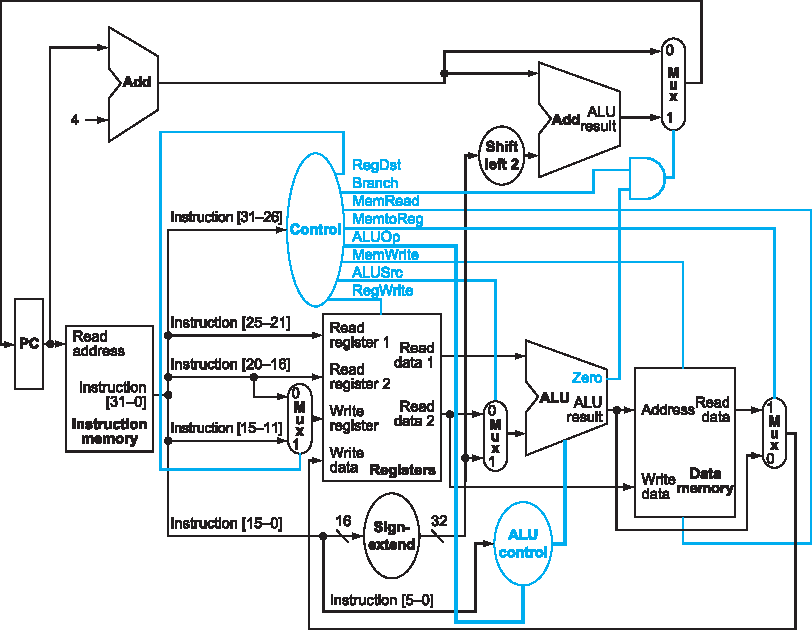
\includegraphics[width=\textwidth]{simple-mips-datapath.pdf}
\end{document}
